\begin{figure}[h]
    \centering
    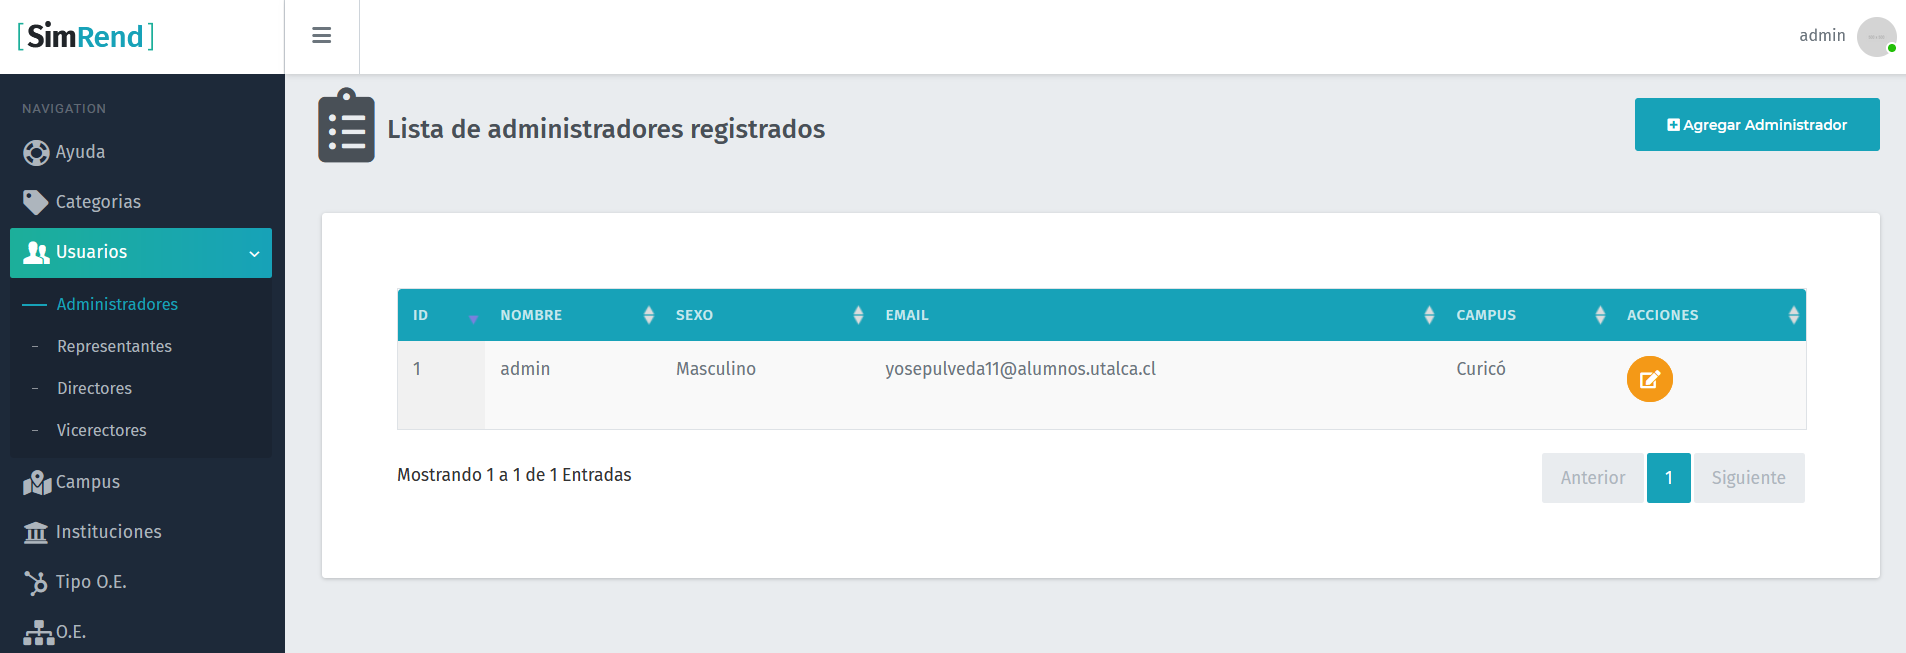
\includegraphics[width=1\textwidth]{Imagenes/CRUDAdministrador.PNG}
    \caption{\label{fig: CRUDAdministrador}Vista para gestionar a los usuarios administradores.}
\end{figure}

\begin{figure}[h]
    \centering
    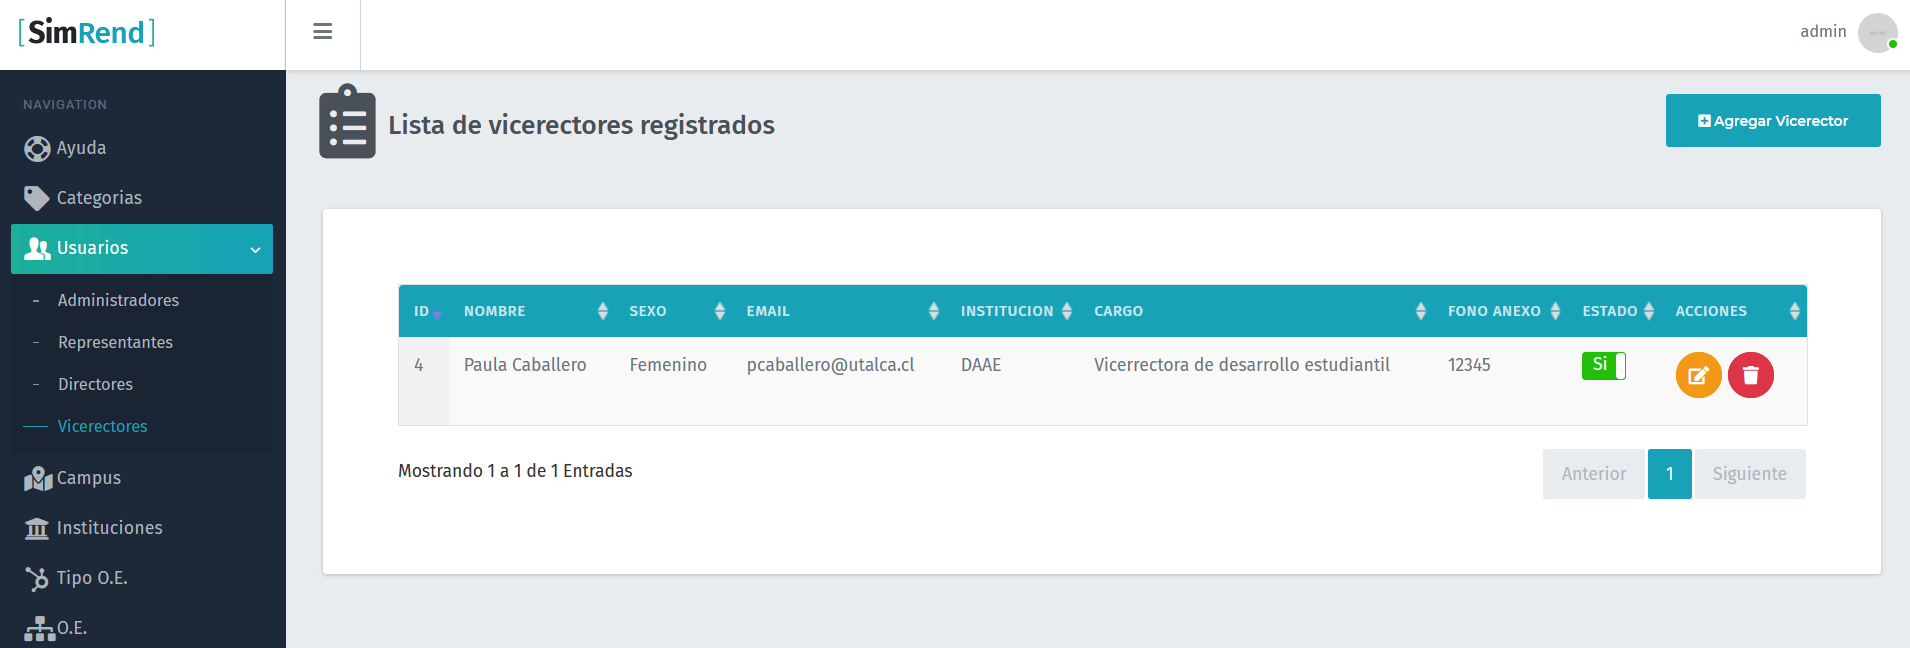
\includegraphics[width=1\textwidth]{Imagenes/CRUDVicerrectores.PNG}
    \caption{\label{fig: CRUDVicerrectores}Vista para gestionar a los usuarios vicerectores.}
\end{figure}

\begin{figure}[h]
    \centering
    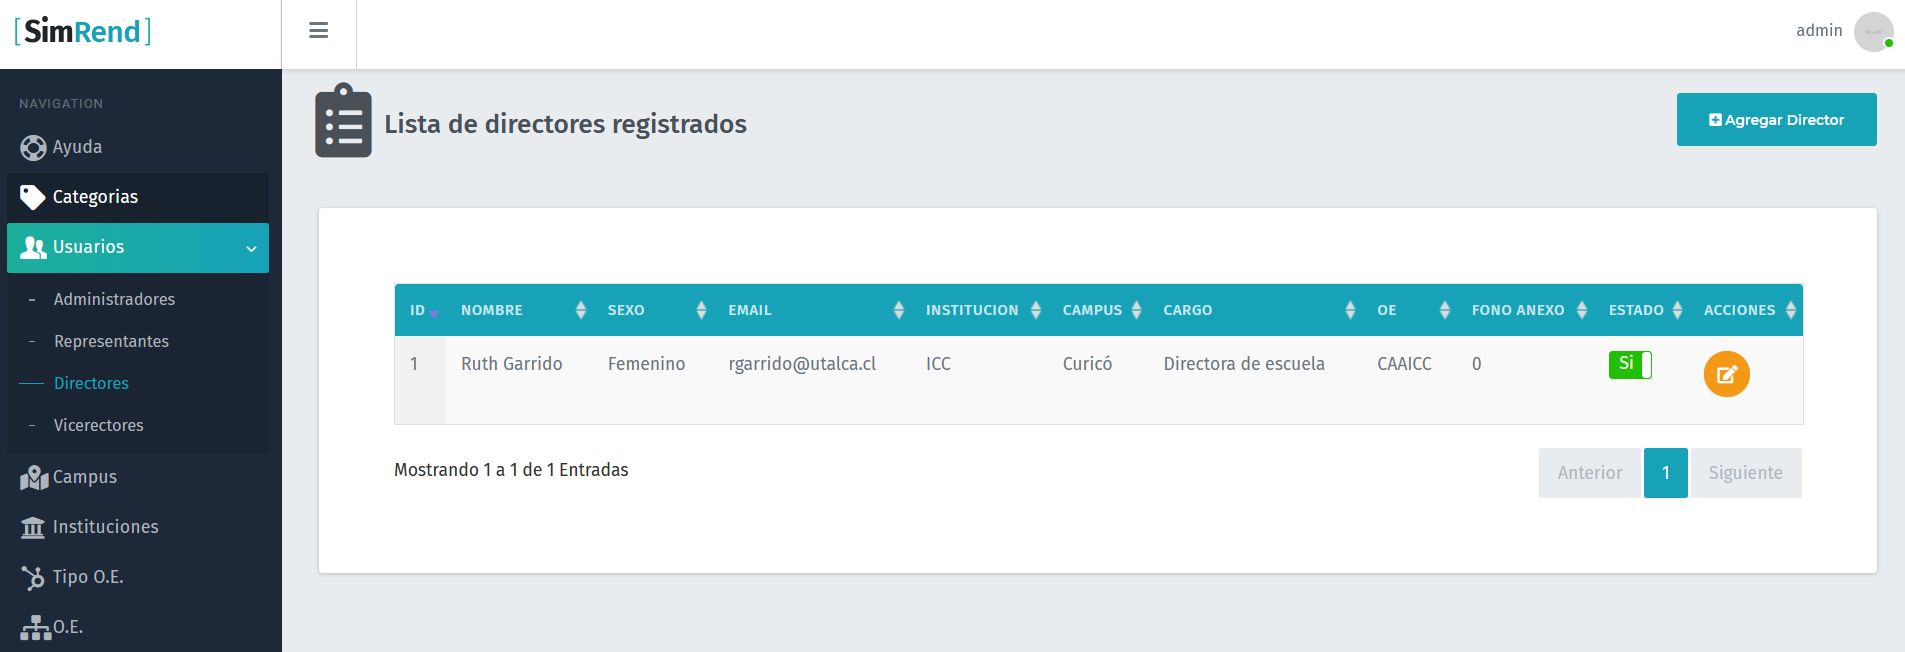
\includegraphics[width=1\textwidth]{Imagenes/CRUDDirectores.PNG}
    \caption{\label{fig: CRUDDirectores}Vista para gestionar a los usuarios directores.}
\end{figure}

\begin{figure}[h]
    \centering
    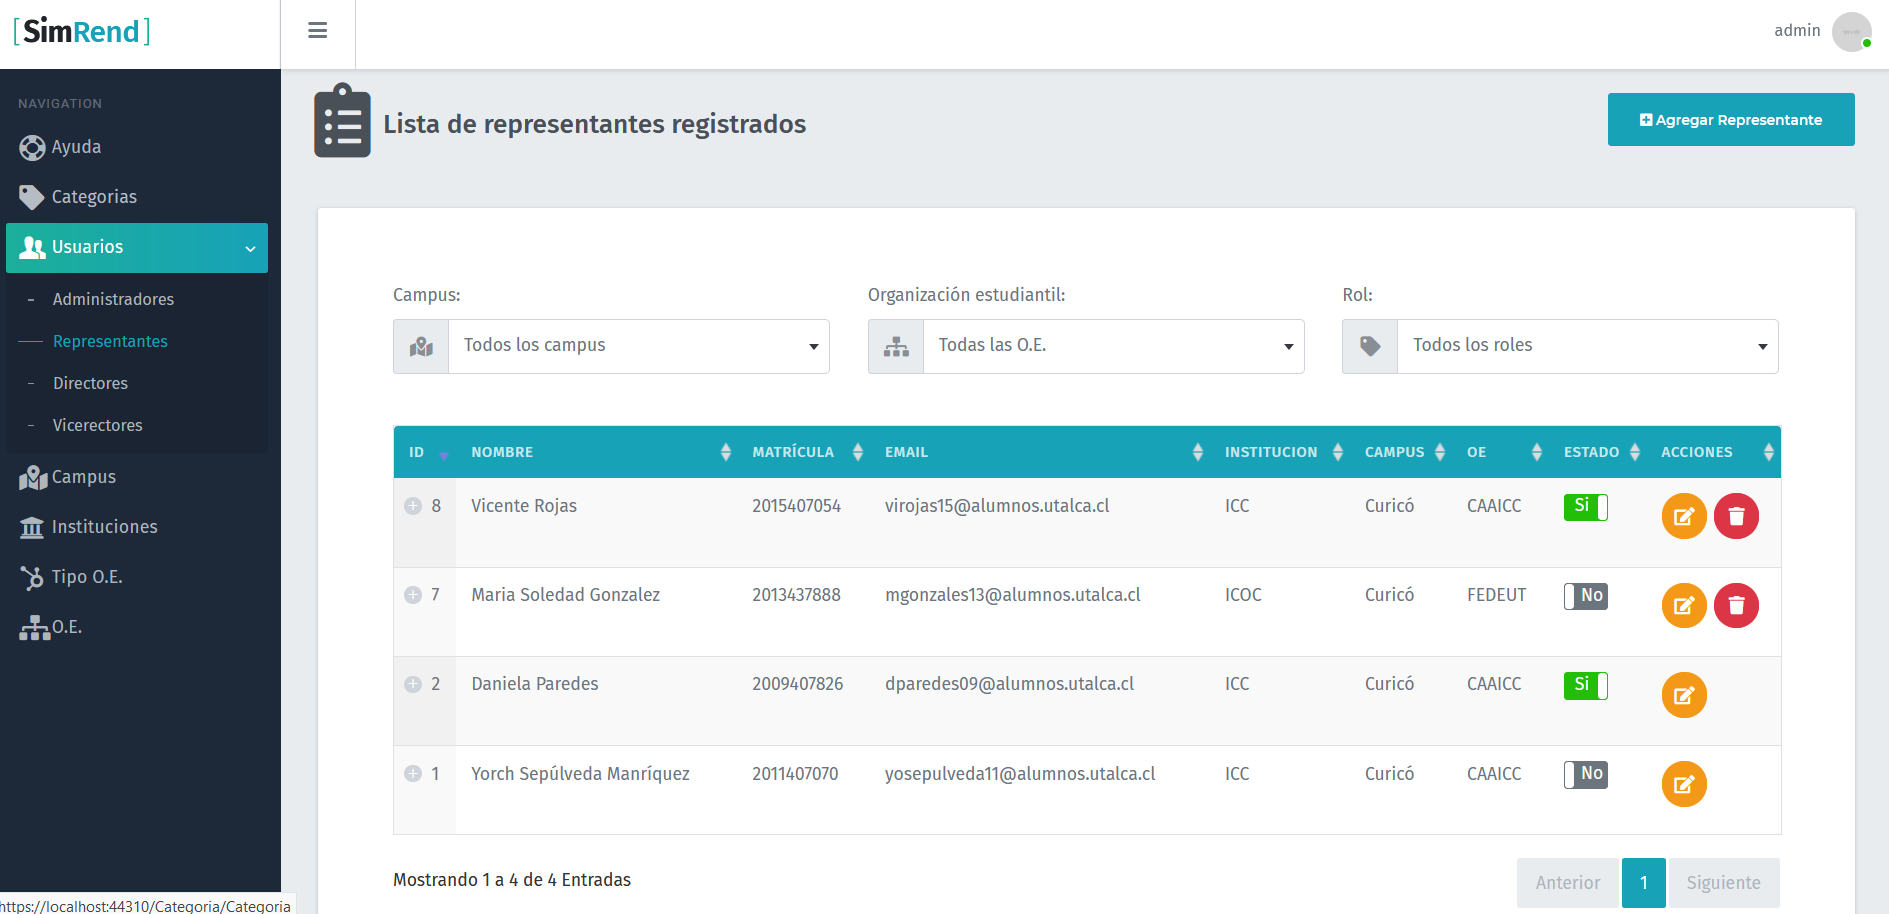
\includegraphics[width=1\textwidth]{Imagenes/CRUDRepresentante.PNG}
    \caption{\label{fig: CRUDRepresentante}Vista para gestionar a los usuarios representates.}
\end{figure}

\begin{figure}[h]
    \centering
    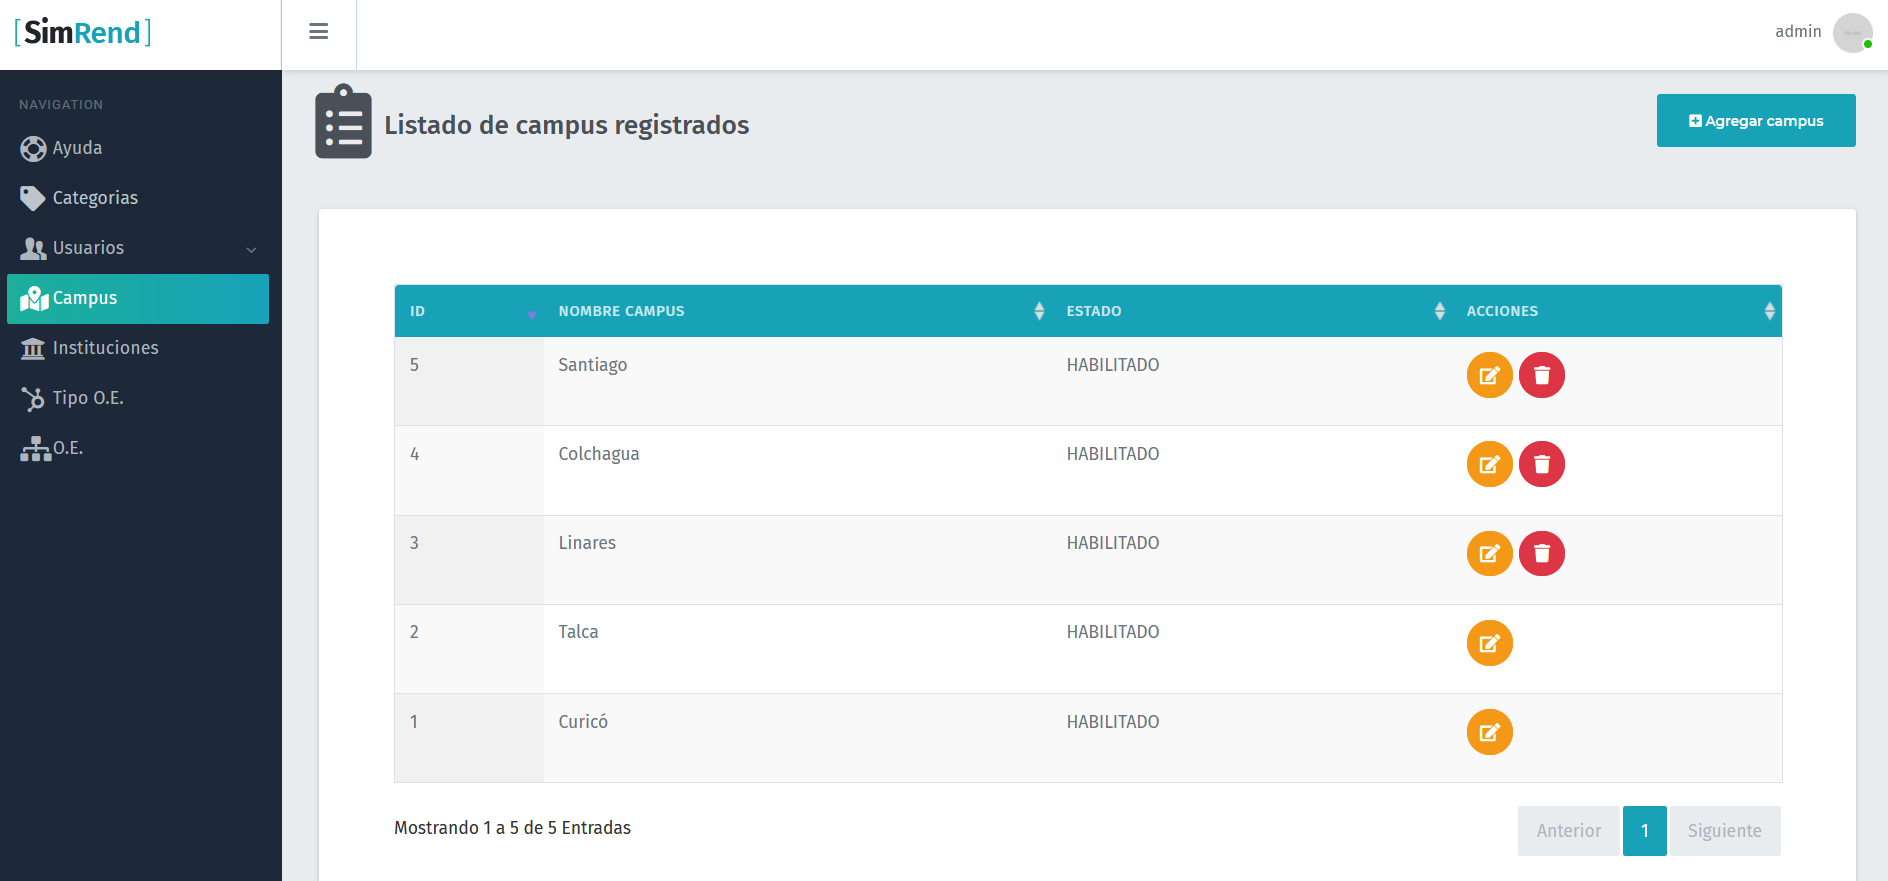
\includegraphics[width=1\textwidth]{Imagenes/CRUDCampus.PNG}
    \caption{\label{fig: CRUDCampus}Vista para gestionar a los distintos campus perteneciente a la Universidad.}
\end{figure}

\begin{figure}[h]
    \centering
    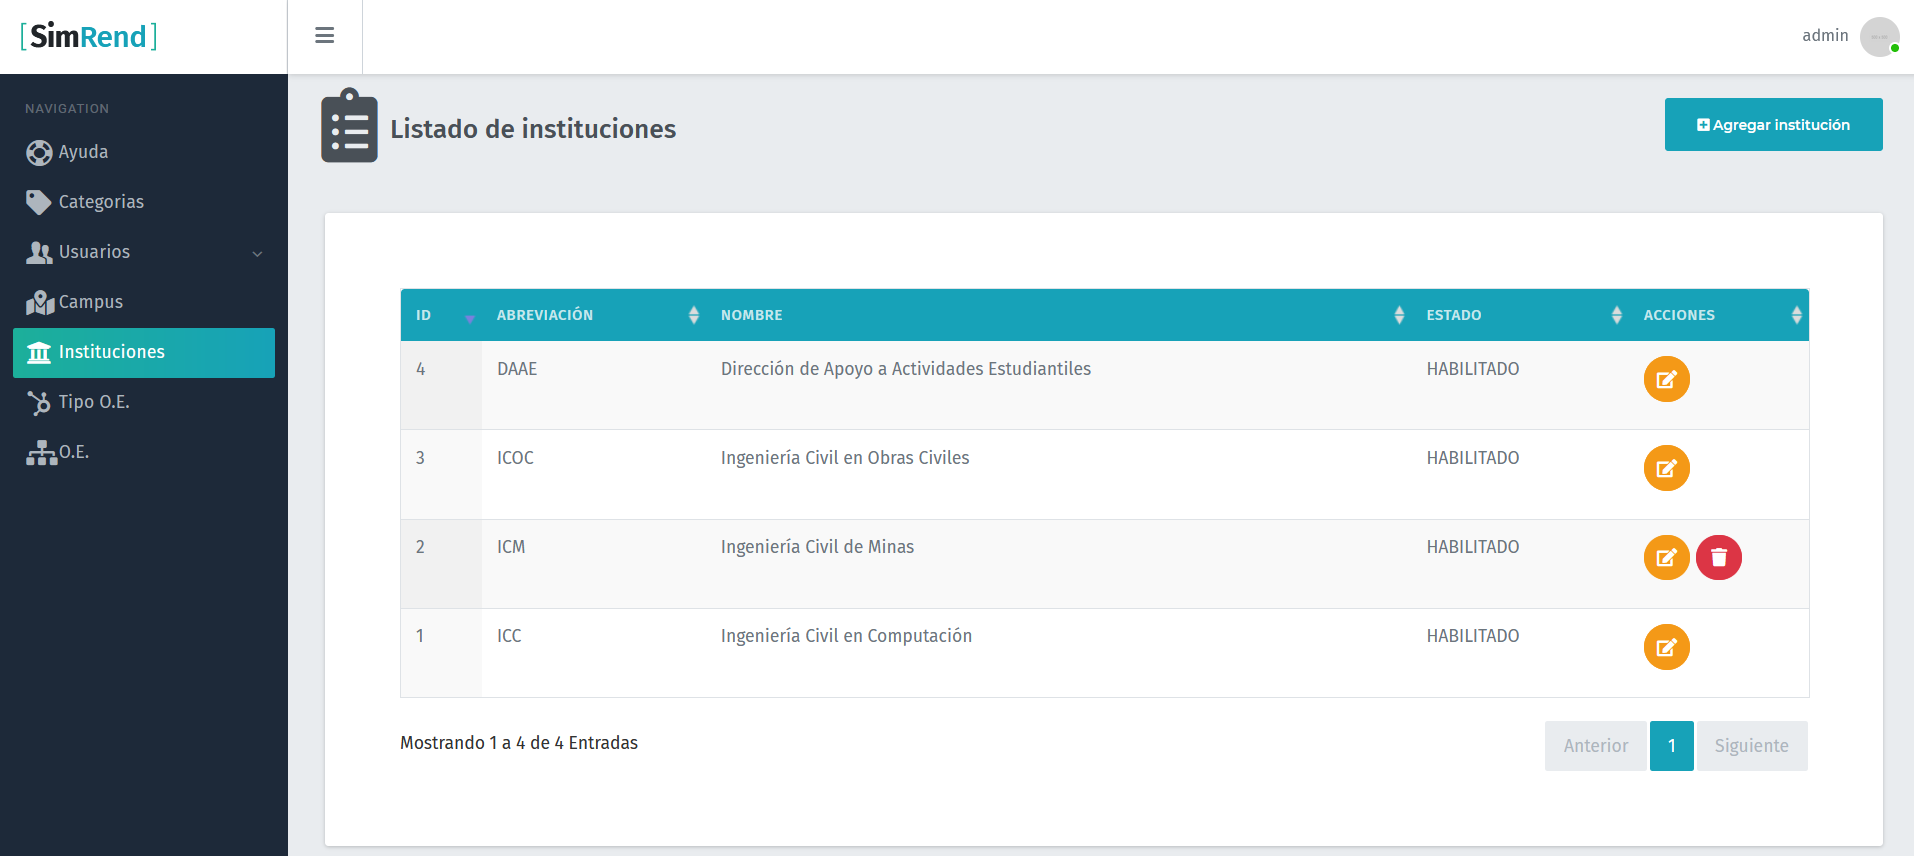
\includegraphics[width=1\textwidth]{Imagenes/CRUDInstituciones.PNG}
    \caption{\label{fig: CRUDInstituciones}Vista para gestionar las distintas instituciones perteneciente a la Universidad.}
\end{figure}

\begin{figure}[h]
    \centering
    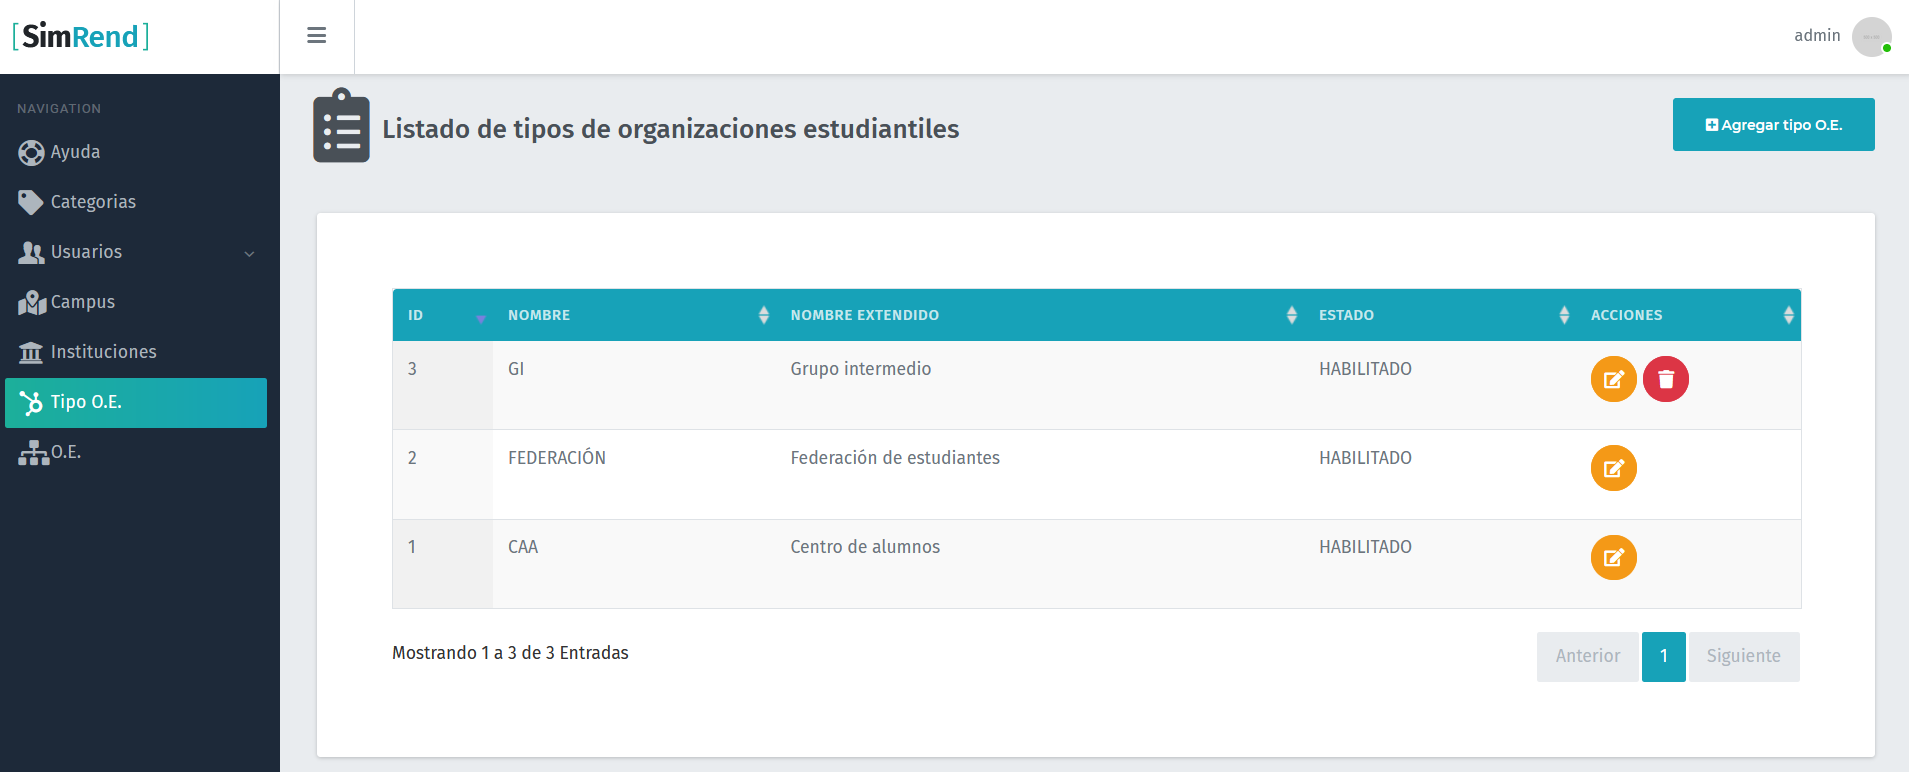
\includegraphics[width=1\textwidth]{Imagenes/CRUDTipoOE.PNG}
    \caption{\label{fig: CRUDTipoOE}Vista para gestionar las distintos tipos de OE perteneciente a la Universidad.}
\end{figure}

\begin{figure}[h]
    \centering
    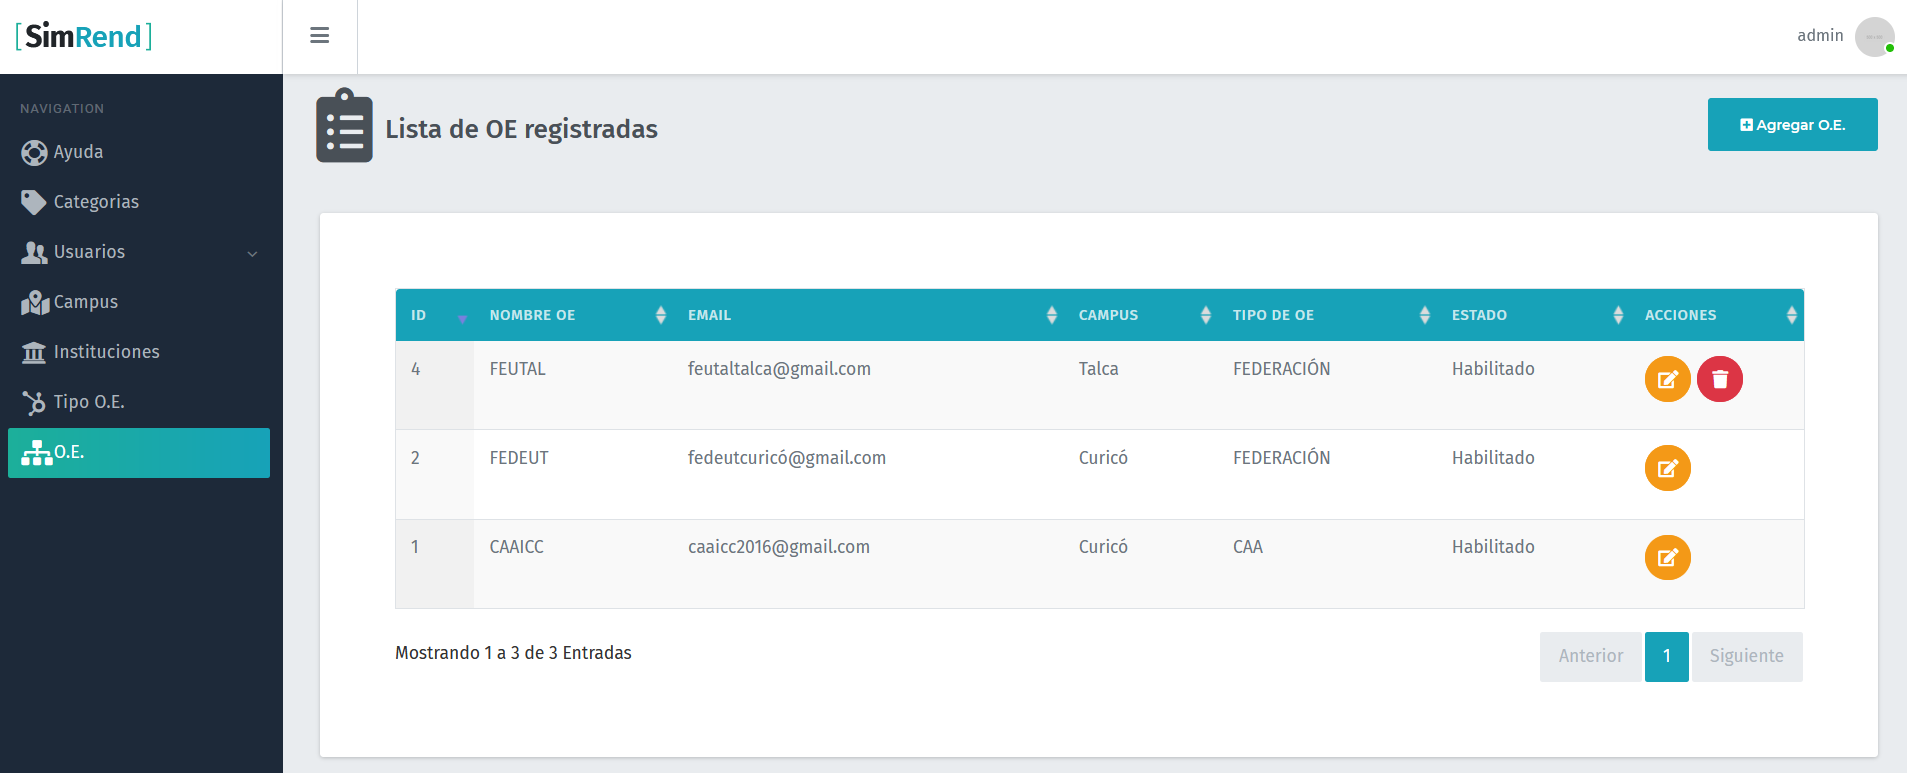
\includegraphics[width=1\textwidth]{Imagenes/CRUDOE.PNG}
    \caption{\label{fig: CRUDOE}Vista para gestionar las distintas OE perteneciente a la Universidad.}
\end{figure}

\begin{figure}[h]
    \centering
    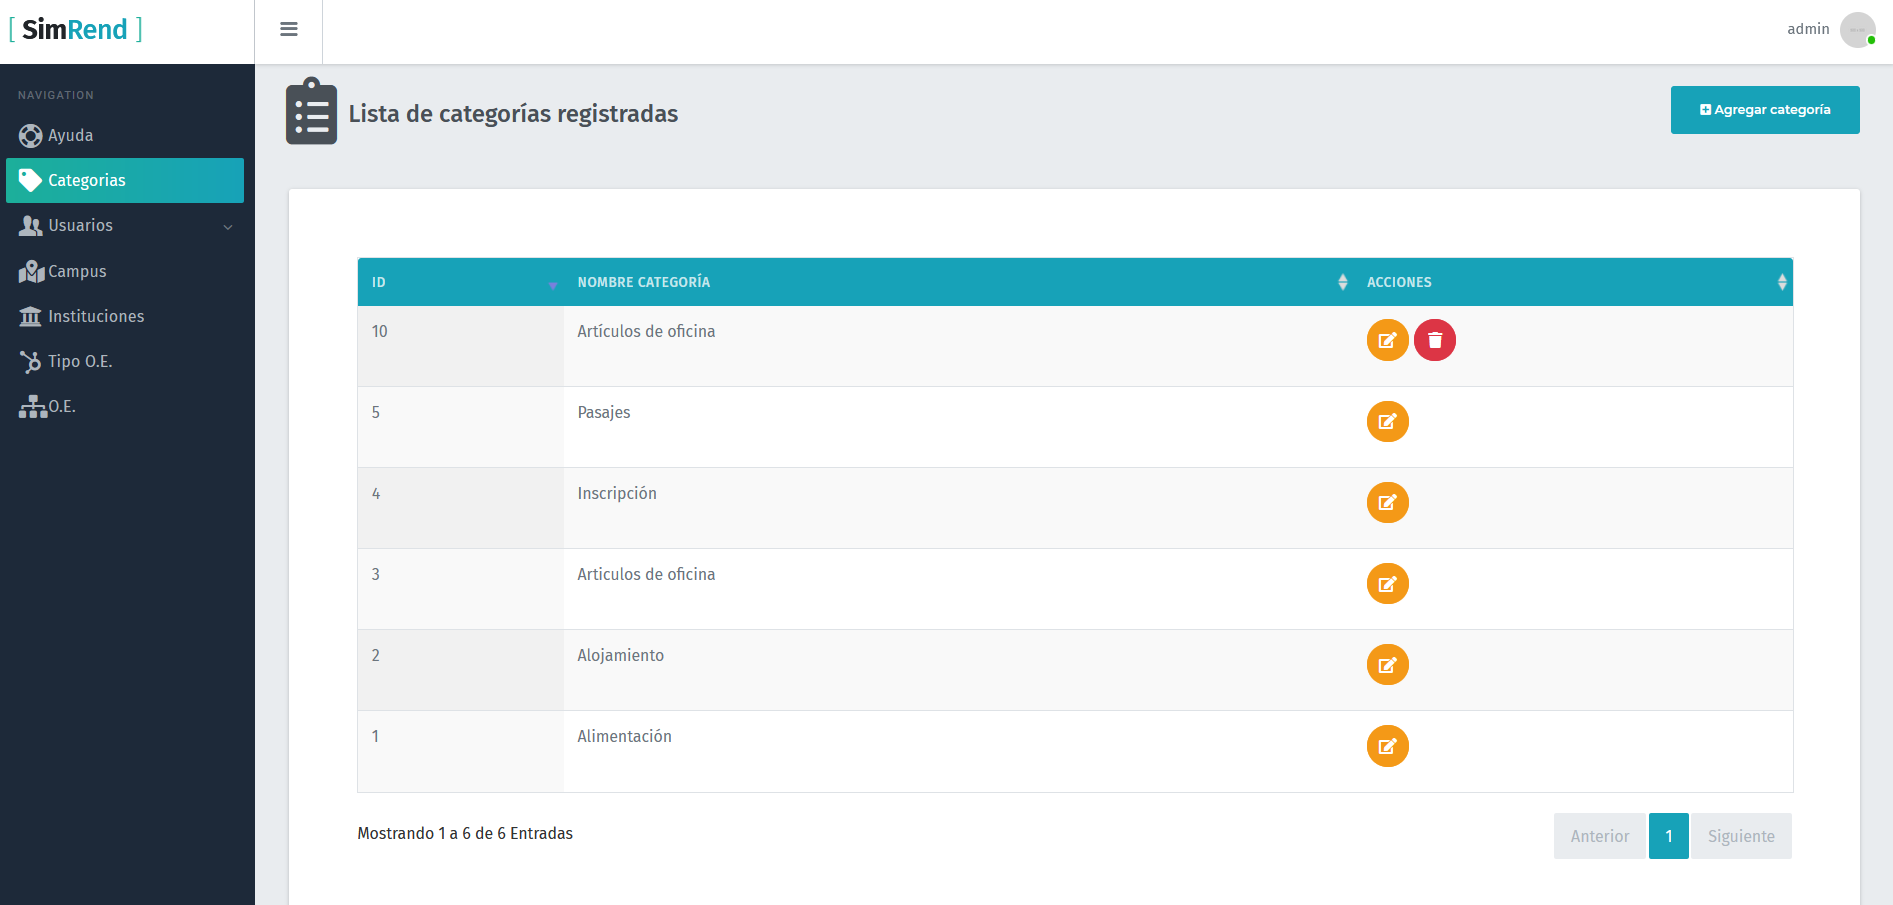
\includegraphics[width=1\textwidth]{Imagenes/CRUDCategoria.PNG}
    \caption{\label{fig: CRUDCategoria}Vista para gestionar las categorías para ser utilizadas en una solicitud de fondos o la respectiva categorización de un documento en la seccion de rendición.}
\end{figure}

\begin{figure}[h]
    \centering
    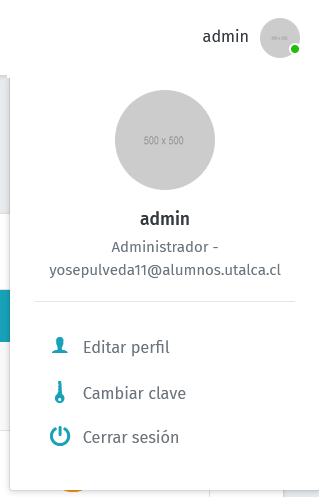
\includegraphics[width=0.5\textwidth]{Imagenes/EditarPerfilClave.PNG}
    \caption{\label{fig: EditarPerfilClave}Botones para acceder a editar el perfil del usuario en sesión o la modificacion de la clave.}
\end{figure}

\begin{figure}[h]
    \centering
    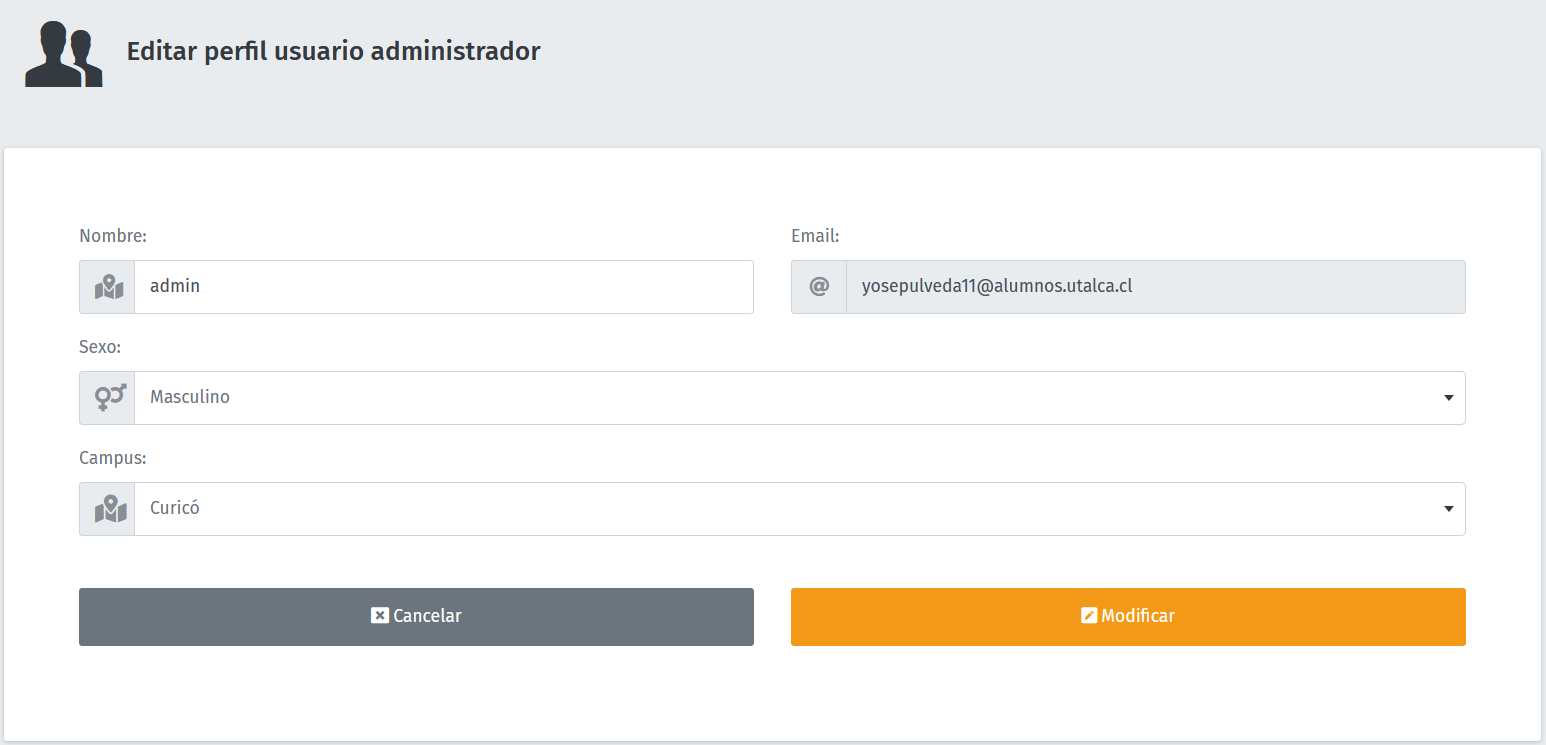
\includegraphics[width=1\textwidth]{Imagenes/EditarPerfil.PNG}
    \caption{\label{fig: EditarPerfil}Vista para modificar los datos del usuario que se encuentra con la sesión iniciada.}
\end{figure}

\begin{figure}[h]
    \centering
    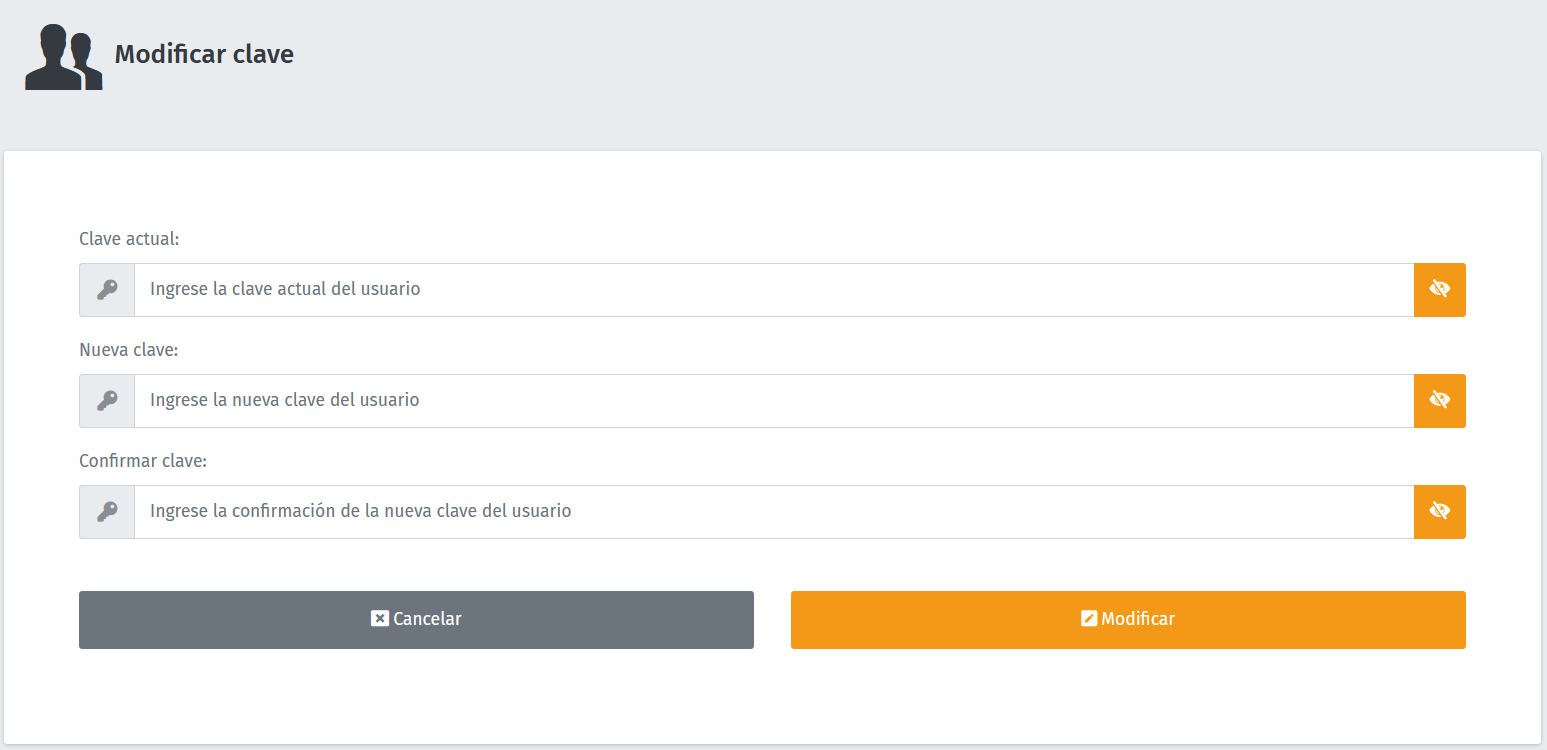
\includegraphics[width=1\textwidth]{Imagenes/ModificarClave.PNG}
    \caption{\label{fig: EditarClave}Vista para modificar la clave del usuario que se encuentra con la sesión iniciada.}
\end{figure}

\begin{figure}[h]
    \centering
    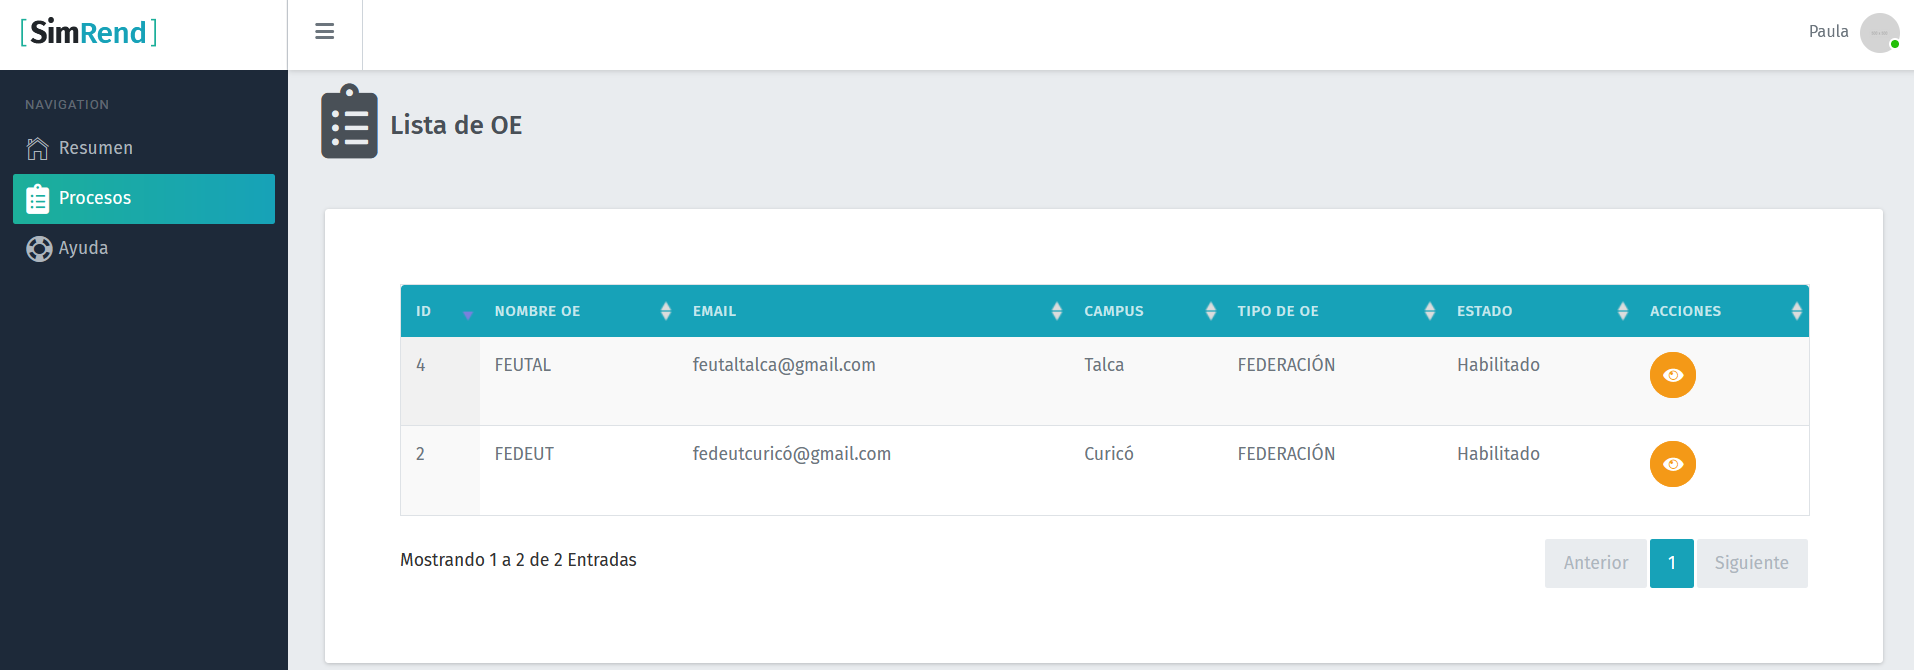
\includegraphics[width=1\textwidth]{Imagenes/PrincipalVicerector.PNG}
    \caption{\label{fig: PrincipalVicerector}Vista principal que visualiza el vicerector, en donde se encuentra un listado de las OE que tiene a su cargo.}
\end{figure}